\documentclass{article}
\usepackage{pgf, tikz}
\usepackage[utf8]{inputenc}
\usepackage{graphicx}
\usepackage{hyperref}

\title{Travail pratique \#3 - IFT-2245}
\author{Nezha Chahid et Dejla Ben Ltaief P1069712} 

\begin{document}
\maketitle
\section {Introduction}
Dans ce travail pratique, nous devons impl\'{e}menter en langage C un programme qui simule un gestionnaire de m\'{e}moire virtuelle par pagination (paging). En
simulant des acc\'{e}s m\'{e}moire cons\'{e}cutifs en traduisant les adresses logiques en adresses physiques de 16 bits.
\section {Impl\'{e}mentation}
\subsection{Lecture}
Nous avons commenc\'{e}e par trouver la page et l'offsset d'une adresse logique donn\'{e}e.
On \'{e}tablit un lookup, si la page se trouve alors le tlb hit  le found count sont est increment\'{e}s.
Si la page n'est pas pr\'{e}sente dans le tlb , alors on cheche dans la table des pages . Si on la trouve page found count et miss count sont  incrementes. Si nous avons un miss et un page fault alors, on fait appel a la fonction demand-page.
Finallement si le TLB est rempli, alors nous utilisons un algorithme de remplacement.
\subsection{Ecriture}
Clairement, c'est la meme implementation qu'on as fait pour la lecture sauf quelques petits changements, Nous ajoutons la sauvegarde du caract\'{e}re a la m\'{e}moire.
\section {r\'{e}ponses aux questions}
\subsection{Question1}
Pour le tlb nous avons utilis\'{e}e deux algorithmes,le premier FIFO, et le second LFU. 
\newline
\begin{enumerate}
\item Algorithme FIFO
\newline Nous avons choisi l'algorithme de remplacement FIFO parce qu'il est tr\'{e}s simple a impl\'{e}menter.
un attribut age a \'{e}t\'{e} ajout\'{e} a la structure, a chaque fois qu'une entr\'{e}e tlb est ajout\'{e} au tlb, ageCounter est increment\'{e}e. si un remplacement doit \^{e}tre fait, on choisit tout simplement celle avec l'age minimale. 
\newline
\newline Avantages du FIFO:
Rapidit\'{e}.
pas de  probl\'{e}me de famine.
\newline
\newline Inconv\`{e}nients  du FIFO:
\newline
il ne prend pas en compte lutilit\`{e} des pages,il prend pas en compte les pages qui sont r\`{e}cemmnent utilis\`{e}es, ni les pages qui sont fr\`{e}quemment utilis\`{e}es, une page qui est utilis\`{e}e une seule fois peut remplacer une page qui est fr\`{e}quement utilis\`{e}e.
\newline Anomalie de Belady : on peut dans certains cas augmenter les  \`{e}changes nec\`{e}ssaires si on augmente la taille de la m\`{e}moire.
\newline 
\item Algorithme LFU
\newline
la moins souvent utilis\`{e}e : on garde un compteur qui est increment\`{e}e  \`{a} chaque fois que le cadre est referenc\`{e}e, et la victime sera le cadre dont le compteur est le plus bas.
Nous l'avons implement\`{e}e de la facon suivante: A chaque fois qu'une entr\`{e}e est ajoute au tlb pour la premi\`{e}re fois, L'attribut use est a 1. A chaque fois que  la variable use est increment\`{e}e. si l'entr\'{e}e sort du TLB table  et elle s'introduit apr\`{e}s ,la variable  use va etre remise a 1.
\newline
Avantages du LFU:
\newline
Facilit\'{e} d'impl\'{e}mentation.
\newline
Inconv\`{e}nients du LFU:
\newline
Cet algorithme pr\`{e}sente un probl\`{e}me quand une page est tr\`{e}s utilis\'{e} pendant la phase initiale d?un programme, mais qu?elle n?est plus employ\`{e}e \`{a} nouveau par la suite. Comme elle a \`{e}t\`{e} amplement utilis\'{e}e, elle poss\'{e}de un grand compte et reste donc en m\`{e}moire m \^{e}me si elle n?est pas utilis\`{e}e.
\end{enumerate}
\subsection{Question2}
Nous avons effectuer quelques modifications au fichier command.in, et nous avons effectu\'{e}e les tests suivants.
\begin{enumerate}
\item \underline{ Fifo applique} 
\newline
\includegraphics{./images/CaptureFIFO.png}
\item \underline{ LFU applique} 
\newline
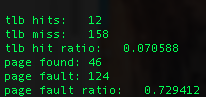
\includegraphics{./images/CaptureLFU.png}
 \item \underline{ Fifo applique} 
 \newline
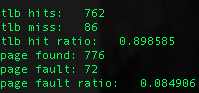
\includegraphics{./images/CaptureFIFO1.png}
 \item \underline{ LFU applique}
 \newline
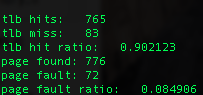
\includegraphics{./images/CaptureLFU1.png}
\end{enumerate}
La pageFault ratio est la m \^{e}me pour les deux algorithmes, ceci est pr \`{e}vu, comme autrefois la page est charg\`{e}e en m\`{e}moire, et que la m\`{e}moire est suffisamment grande pour stocker les donn\`{e}es, alors aucun  \`{e}change doit \^{e}tre effectu \`{e}e.
Par ailleurs nous remarquons une diff\`{e}rnce entre tlb hit ratio pour  LFU est  FIFO dans les deux cas.LFU bat FIFO de 2 pourcent dans le premier test  1 pourcent dans le second test.
Finalement , LFU est plus efficace que FIFO.
\subsection{Question3}
\underline{resultats-FIFO} 
\newline
\underline{Sans les changements}
\newline 
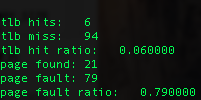
\includegraphics{./images/fifo1.png}
\newline
\underline{Avec les changements}
\newline
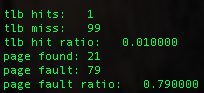
\includegraphics{./images/fifo.png}
\newline
\underline{ Configuration} 
\newline
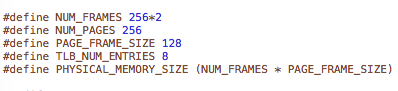
\includegraphics{./images/Fifoconf.png}
Nous avons fait des tests sur 100 elements
D'apr\`{e}s les images ci dessous, nous remarquons que pour l'algorithme fifo que la situation se degrade en modifiant le tlb entries a 8 le tlb-miss est passee de 96 a 99. 
\newline
2 \'{e}me test:
\newline
Nous avons modifi\'{e} le num frames a 512 et le ratio du Fifo a diminu\'{e} , ce qui confirme son incovenient cit\'{e} ci dessus ce qui n'est pas le cas pour LFU ou le hitratio reste le meme.
\newline
\underline{Avec les changements}
\newline
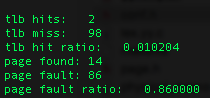
\includegraphics{./images/CaptureAnomalie.png}
\newline
Nous avons essay\'{e} de modifi\'{e} le NUMPAGES en l'augmentant mais nous n'avons pas eu des changements dans les deux cas.
\subsection{References}
\url{http://stic-os.webs.com/Support_Cours/Algorithmes%20de%20remplacement.pdf}
\newline
Un ancien Tp
\newline
Plusieurs notes de cours
\end{document}
